\section{Vektorräume}

\subsection{Kern und Bild}
Der \textbf{Kern}, Nullmenge oder Nullraum $\ker(A) = \{x \in \mathbb{R}^n | A\vec{x} = 0\}$ sind alle Elemente, für die der Funktionswert gleich dem Nullvektor $x$ ($A\vec{x} = 0$) ist. Der Kern ist daher nichts anders als die Lösungsmenge! \\
Beispiel:
\[
	\ker(A) = \begin{pmatrix}
		2 & 2 & -8\\
		0 & 1 &-2 \\
		-1 & 1 & 0
	\end{pmatrix} \cdot \begin{pmatrix}
		x_1\\
		x_2\\
		x_3
	\end{pmatrix} \eqi \begin{pmatrix}
		0\\
		0\\ 
    	0
\end{pmatrix} 
\]

\noindent Der Kern von Abbildung $A$ ist $\ker(A) = \lambda\begin{pmatrix}2 \\ 2 \\ 1\end{pmatrix}$.

\noindent Das \textbf{Bild} oder auch Bildraum ist die Menge aller Linearkombinationen der Spaltenvektoren $\im(A) = \{Bt | t \in \mathbb{R}^m\}$.


\subsection{Basis}
Um die Abbildung $A$ in eine andere Basis $A'$ (bzw. Koordinaten-System) umzurechnen kann folgendes verwendet werden: \\
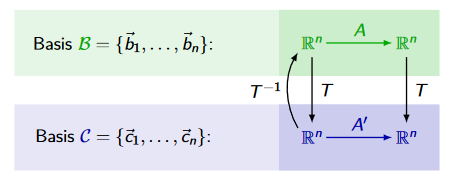
\includegraphics[width=\columnwidth]{./Images/Basiswechsel.png}

\noindent $A' = TAT^{-1}$ Siehe auch \verweiseref{basistransformation} um $T$ zu berechnen. 

\subsection{Basistransformation}\label{basistransformation}
\noindent Koordinaten $I$ in der Basis $B$ in die neue Koordinaten $I'$ in der Basis $B'$ berechnen. Die Transformationsmatrix $T$ kann für beliebige Umwandlungen verwendet werden.
\[
\begin{array}{|ccc|ccc|}
	\hline
	I'_1 & \dots & I'_n & I_1 & \dots & I_n \\
	\hline
	& & & & &\\
	& & & & &\\
	& & & & &\\
	& B' & & & B &\\
	& & & & &\\
	& & & & &\\
	& & & & &\\
	\hline
\end{array}
\xrightarrow{Gauss}
\begin{array}{|ccc|ccc|}
	\hline
	I'_1 & \dots & I'_n & I_1 & \dots & I_n \\
	\hline
	1 & \dots & 0 & & &\\
	\vdots & \ddots & \vdots & & T  &\\
	0 & \dots & 1 & & & \\ \hline
	0 & \dots & 0 & & &\\
	\vdots & \ddots & \vdots & & \textcolor{red}{*}  &\\
	0 & \dots & 0 & & & \\
	\hline
\end{array}
\]

\noindent\textcolor{red}{*} = 0 ist gleichbedeutend damit, dass die Koordinaten umgerechnet werden können.

\subsubsection{Drehmatrix}
Eine Drehmatrix $M$ ist immer orthogonal (\verweiseref{orthogonalmatrix}) und hat die Determinante $\det(M) = 1$.\\

\noindent
Sie wird gefunden, indem 3 \textit{beliebige} Punkte auf einer Abbildung vor ($P$) und nach ($P'$) der Drehung markiert werden und mithilfe von $D = P'P^{-1}$ berechnet. \textit{$P$ und $P'$ muss regulär (Linearunabhängig) sein $\rightarrow$ sonst andere Koordinaten verwenden}!
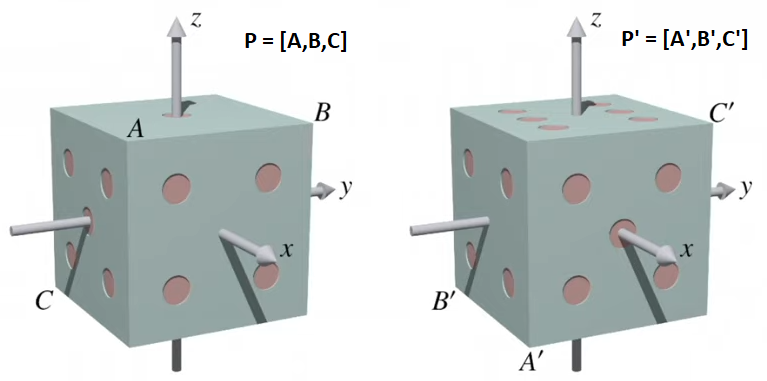
\includegraphics[width=\columnwidth]{./Images/Drehmatrix.png}

\noindent
Um den Drehwinkel $\alpha$ zu berechnen, kann die \textit{Spur} einer Matrix verwendet werden. (Siehe \verweiseref{drehwinkel})

\subsection{Volumen}\label{gram-determinante}
Mittels der \textbf{Gram-Determinante} kann ein Volumen $V$ in $\mathbb{R}^n$ Dimension berechnet werden. In der $\mathbb{R}^2$ Dimension ergibt dies die Fläche!

\begin{align*}
	V = \text{Gram}(a_1, a_2) &= \begin{vmatrix}
		\vec{a}_1 \circ \vec{a}_1 & \vec{a}_1 \circ \vec{a}_2 \\
		\vec{a}_2 \circ \vec{a}_1 & \vec{a}_2 \circ \vec{a}_2 \\
	\end{vmatrix} \\
	\vec{b}_1 = \frac{\vec{a}_1}{|\vec{a}_1|} \Rightarrow &= |\vec{a}_1| \cdot \begin{vmatrix}
		\vec{b}_1 \circ \vec{a}_1 & \vec{b}_1 \circ \vec{a}_2 \\
		\vec{a}_2 \circ \vec{a}_1 & \vec{a}_2 \circ \vec{a}_2 \\
	\end{vmatrix} \\
	\vec{b}_2 = \frac{\vec{a}_2 - (\vec{b}_1 \circ \vec{a}_2)\vec{b}_1}{l} \Rightarrow &=  |\vec{a}_1| \cdot l \cdot \begin{vmatrix}
		\vec{b}_1 \circ \vec{a}_1 & \vec{b}_1 \circ \vec{a}_2 \\
		\vec{b}_2 \circ \vec{a}_1 & \vec{b}_2 \circ \vec{a}_2 \\
	\end{vmatrix} \\
	&= |\vec{a}_1|^2 \cdot l^2 \cdot \underbrace{\begin{vmatrix}
		\vec{b}_1 \circ \vec{b}_1 & \vec{b}_1 \circ \vec{b}_2 \\
		\vec{b}_2 \circ \vec{b}_1 & \vec{b}_2 \circ \vec{b}_2 \\
	\end{vmatrix}}_{\det(E) = 1} \\
	&=  |\vec{a}_1|^2 \cdot l^2  = \text{Fläche}(\vec{a}_1, \vec{a}_2)^2
\end{align*}

\begin{align*}
	\det(M) = \left\lbrace
	\begin{array}{r@{}l}
		> 0, & {}\qquad Rechtssystem \\
		< 0, & {}\qquad Linkssystem
	\end{array}
	\right.
\end{align*}

\begin{center}
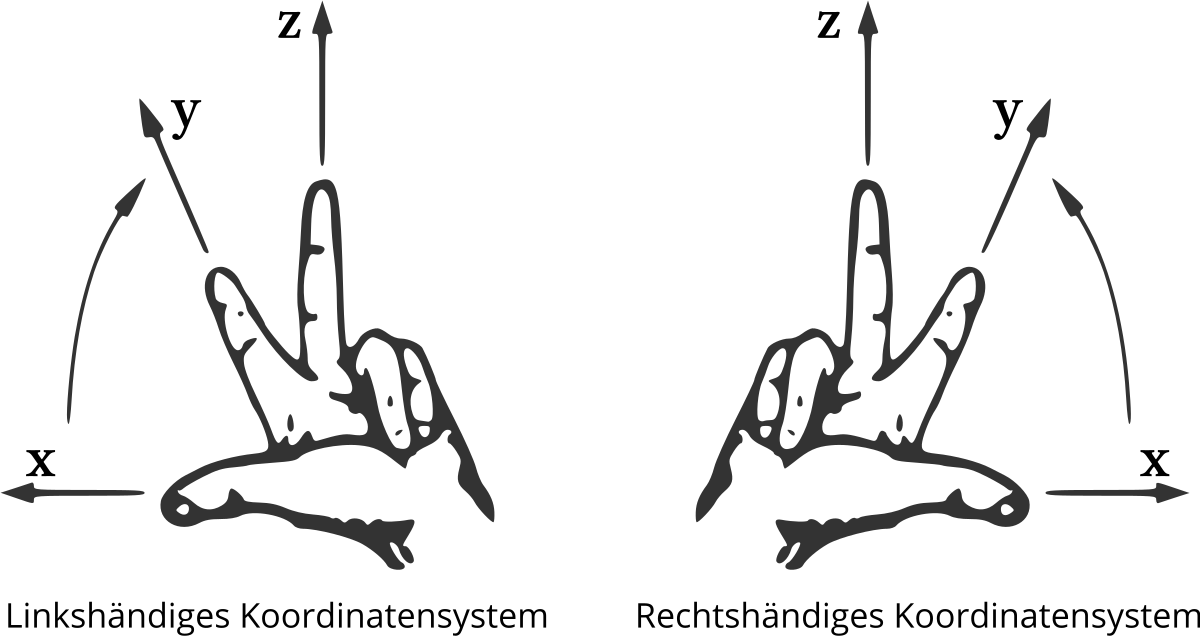
\includegraphics[height=80pt]{./Images/Koordinatensysteme.png}
\end{center}
